\documentclass[]{IEEEtran}
% some very useful LaTeX packages include:
%\usepackage{cite}      
\usepackage{graphicx}   
\usepackage{subfigure} 
\usepackage{url}       
\usepackage{amsmath}    
\usepackage{caption2}
% Your document starts here!
\begin{document}

% Define document title and author
	\title{Weekly Report}
	\author{Adviser: Prof. Yang Wen \\Student: Cheng Wensheng\\ Period: 2018.4.27-5.4
	}
	\markboth{Visual Information Processing Group}{}
	\maketitle

% Write abstract here
\begin{abstract}
	This week I mainly put my effort on reading the classic CNN-based semantic segmentation framework SegNet.
\end{abstract}

% Each section begins with a \section{title} command
\section{Paper outline}
	% \PARstart{}{} creates a tall first letter for this first paragraph
	\PARstart{A}{fter} the pioneering work of Fully Convolutional Networks(FCN), SegNet has been proposed as the best segmentation framework at that time. Its main contributions are as follows.
	\begin{itemize}
		\item Proposed a new decoder network to map the low resolution encoder feature maps to full input resolution feature maps for pixel-wise classification. The novelty of SegNet lies is in the manner in which the decoder upsamples its lower resolution input feature map(s). 
		\item Specifically, the decoder uses pooling indices computed in the max-pooling step of the corresponding encoder to perform non-linear upsampling. This eliminates the need for learning to upsample.  
		\item The upsampled maps are sparse and are then
		convolved with trainable filters to produce dense feature maps.
	\end{itemize}

\section{conclusion}
% \PARstart{}{} creates a tall first letter for this first paragraph
	The author did corresponding experiments to compare SegNet with other state-of-the-art frameworks, analyzed results and got the following conclusion.

	Those architectures which store the encoder
	network feature maps in full perform best but consume more
	memory during inference time. SegNet on the other hand is
	more efficient since it only stores the max-pooling indices of
	the feature maps and uses them in its decoder network to
	achieve good performance.
		
	Fig.~\ref{fig:mp} is the overall framework. Fig.~\ref{fig:ss} is the output of semantic segmentation.
\newpage
\begin{figure}[!hbt]
%		 Center the figure.
		\vspace{2.3cm}
%		\hspace{50cm}
		\begin{center}
			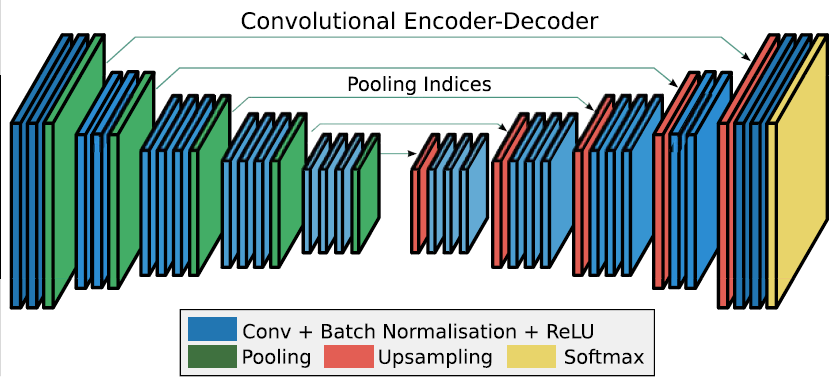
\includegraphics[width=\columnwidth]{fw}
				%		 Create a subtitle for the figure.
			\caption{Framework}
			\label{fig:mp}
		    \hspace{0.5cm}
			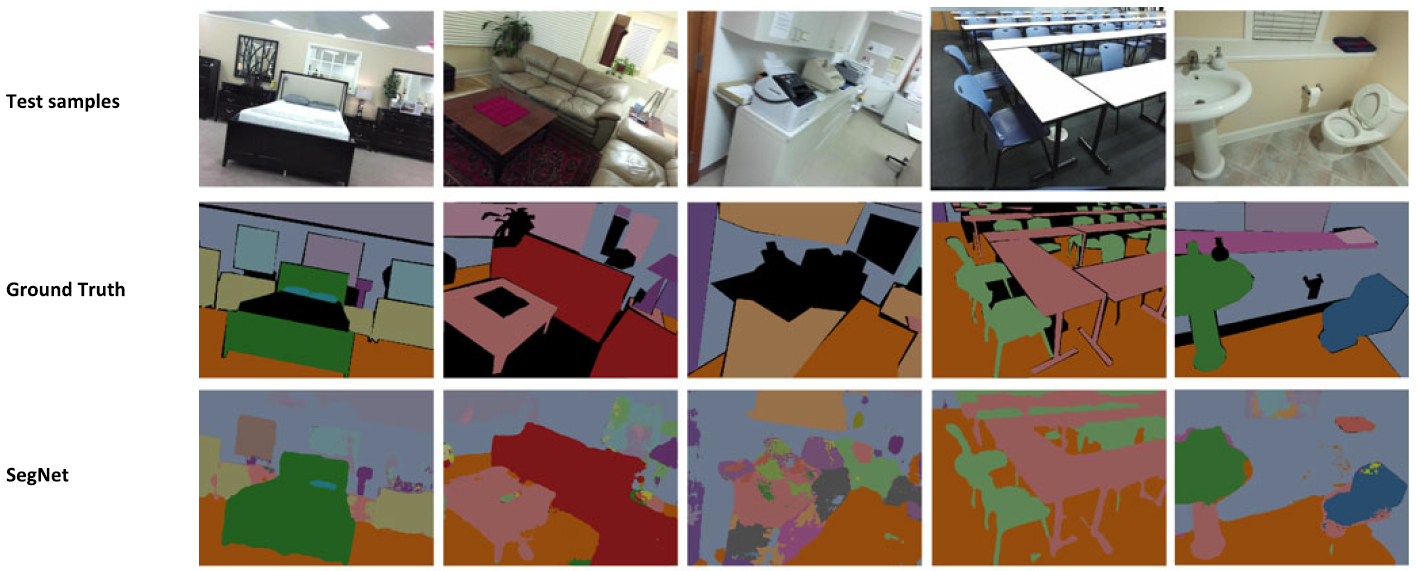
\includegraphics[width=\columnwidth]{rs}
				%Create a subtitle for the figure.
			\caption{Semantic segmentation results}
			\label{fig:ss}
		\end{center}
	\end{figure}

% Now we need a bibliography:
%\begin{thebibliography}{5}
%
%	%Each item starts with a \bibitem{reference} command and the details thereafter.
%	\bibitem{HOP96} % Transaction paper
%	J.~Hagenauer, E.~Offer, and L.~Papke. Iterative decoding of binary block
%	and convolutional codes. {\em IEEE Trans. Inform. Theory},
%	vol.~42, no.~2, pp.~429–-445, Mar. 1996.
%
%	\bibitem{MJH06} % Conference paper
%	T.~Mayer, H.~Jenkac, and J.~Hagenauer. Turbo base-station cooperation for intercell interference cancellation. {\em IEEE Int. Conf. Commun. (ICC)}, Istanbul, Turkey, pp.~356--361, June 2006.
%
%	\bibitem{Proakis} % Book
%	J.~G.~Proakis. {\em Digital Communications}. McGraw-Hill Book Co.,
%	New York, USA, 3rd edition, 1995.
%
%	\bibitem{talk} % Web document
%	F.~R.~Kschischang. Giving a talk: Guidelines for the Preparation and Presentation of Technical Seminars.
%	\url{http://www.comm.toronto.edu/frank/guide/guide.pdf}.
%
%	\bibitem{5}
%	IEEE Transactions \LaTeX and Microsoft Word Style Files.
%	\url{http://www.ieee.org/web/publications/authors/transjnl/index.html}
%
%\end{thebibliography}

% Your document ends here!
\end{document}